% -*- compile-command: "cd ../ && make" -*-
\eocesolch{Foundations for inference}
\begin{multicols}{2}

% 1

\eocesol{(a)~Mean. Each student reports a numerical value: a number of hours.
(b)~Mean. Each student reports a number, which is a percentage, and we can
average over these percentages.
(c)~Proportion. Each student reports Yes or No, so this is a categorical
variable and we use a proportion.
(d)~Mean. Each student reports a number, which is a percentage like in part~(b).
(e)~Proportion. Each student reports whether or not s/he expects to get a job,
so this is a categorical variable and we use a proportion.}

% 3

\eocesol{(a)~Mean: 13.65. Median:~14.
(b)~SD: 1.91. IQR: $15-13=2$.
(c)~$Z_{16} = 1.23$, which is not unusual since it is within 2~SD of the mean.
$Z_{18} = 2.28$, which is generally considered unusual.
(d)~No. Point estimates that are based on samples only approximate the
population parameter, and they vary from one sample to another.
(e)~We use the SE, which is $1.91/\sqrt{100} = 0.191$ for this sample's mean.}

% 5

\eocesol{(a)~We are building a distribution of sample statistics, in this case the sample
mean. Such a distribution is called a sampling distribution.
(b)~Because we are dealing with the distribution of sample means, we need to
check to see if the Central Limit Theorem applies. Our sample size is greater
than 30, and we are told that random sampling is employed. With these conditions
met, we expect that the distribution of the sample mean will be nearly normal
and therefore symmetric.
(c)~Because we are dealing with a sampling distribution, we measure its
variability with the standard error. $SE = 18.2 / \sqrt{45} = 2.713$.
(d)~The sample means will be more variable with the smaller sample size.}

% 7

\eocesol{Recall that the general formula is
\begin{align*}
\text{point estimate} \pm Z^{\star} \times SE
\end{align*}
First, identify the three different values. The point estimate is 45\%,
$Z^{\star} = 1.96$ for a 95\% confidence level, and $SE = 1.2\%$. Then, plug the
values into the formula:
\begin{align*}
45\% \pm 1.96 \times 1.2\% \quad\to\quad (42.6\%, 47.4\%)
\end{align*}
We are 95\% confident that the proportion of US adults who live with one or more
chronic conditions is between 42.6\% and 47.4\%.}

% 9

\eocesol{(a)~False. Confidence intervals provide a range of plausible values, and
sometimes the truth is missed. A 95\% confidence interval ``misses'' about 5\%
of the time.
(b)~True. Notice that the description focuses on the true population value.
(c)~True. If we examine the 95\% confidence interval computed in Exercise~\ref{chronic_illness_tf}, we can see that 50\% is not included in this interval. This
means that in a hypothesis test, we would reject the null hypothesis that the
proportion is~0.5.
(d)~False. The standard error describes the uncertainty in the overall estimate
from natural fluctuations due to randomness, not the uncertainty corresponding
to individuals' responses.}

% 11

\eocesol{(a)~We are 95\% confident that Americans spend an average of 1.38 to 1.92 hours
per day relaxing or pursuing activities they enjoy.
(b)~Their confidence level must be higher as the width of the confidence
interval increases as the confidence level increases.
(c)~The new margin of error will be smaller since as the sample size increases
the standard error decreases, which will decrease the margin of error.}


\textC{
\end{multicols}
\newpage
\begin{multicols}{2}
}


% 13

\eocesol{(a)~False. Provided the data distribution is not very strongly skewed ($n = 64$ in
this sample, so we can be slightly lenient with the skew), the sample mean will
be nearly normal, allowing for the method normal approximation described.
(b)~False. Inference is made on the population parameter, not the point
estimate. The point estimate is always in the confidence interval.
(c)~True.
(d)~False. The confidence interval is not about a sample mean.
(e)~False. To be more confident that we capture the parameter, we need a wider
interval. Think about needing a bigger net to be more sure of catching a fish in
a murky lake.
(f)~True. Optional explanation: This is true since the normal model was used to
model the sample mean. The margin of error is half the width of the interval,
and the sample mean is the midpoint of the interval.
(g)~False. In the calculation of the standard error, we divide the standard
deviation by the square root of the sample size. To cut the SE (or margin of
error) in half, we would need to sample $2^2 = 4$ times the number of people in
the initial sample.}

% 15

\eocesol{Independence: sample from $<10\%$ of population, and it is a random sample. We
can assume that the students in this sample are independent of each other with
respect to number of exclusive relationships they have been in. Notice that
there are no students who have had no exclusive relationships in the
sample, which suggests some student responses are likely missing (perhaps only
positive values were reported). The sample size is at least 30. The skew is
strong, but the sample is very large so this is not a concern. 90\% CI: (2.97, 3.43).
We are 90\% confident that undergraduate students have been in 2.97 to 3.43 exclusive relationships, on average.}

% 17

\eocesol{(a)~$H_0: \mu = 8$ (On average, New Yorkers sleep 8 hours a night.) \\
$H_A: \mu < 8$ (On average, New Yorkers sleep less than 8 hours a night.) \\
(b)~$H_0: \mu = 15$ (The average amount of company time each employee spends not
working is 15 minutes for March Madness.) \\
$H_A: \mu > 15$ (The average amount of
company time each employee spends not working is greater than 15 minutes for
March Madness.)}

% 19

\eocesol{The hypotheses should be about the population mean ($\mu$), not the sample mean.
The null hypothesis should have an equal sign and the alternative hypothesis
should be about the null hypothesized value, not the observed sample mean.
Correction:
\begin{align*}
H_0&: \mu = 10~hours \\
H_A&: \mu > 10~hours
\end{align*}
The one-sided test indicates that we are only interested in showing that 10 is an
underestimate. Here the interest is in only one direction, so a one-sided test
seems most appropriate. If we would also be interested if the data showed strong
evidence that 10 was an overestimate, then the test should be two-sided.}

% 21

\eocesol{(a)~This claim does is not supported since 3 hours (180 minutes) is not in
the interval.
(b)~2.2~hours (132 minutes) is in the 95\% confidence interval, so we do not
have evidence to say she is wrong. However, it would be more appropriate to use
the point estimate of the sample.
(c)~A 99\% confidence interval will be wider than a 95\% confidence interval,
meaning it would enclose this smaller interval. This means 132 minutes would be
in the wider interval, and we would not reject her claim based on a 99\%
confidence level.}

% 23

\eocesol{$H_0: \mu = 130$. $H_A: \mu \ne 130$. $Z=1.39$ $\to$ p-value $= 0.1646$, which
is larger than $\alpha=0.05$. The data do not provide convincing evidence that
the true average calorie content in bags of potato chips is different than 130
calories.}

% 25

\eocesol{(a)~Independence: The sample is random and 64 patients would almost certainly
make up less than 10\% of the ER residents. The sample size is at least 30. No
information is provided about the skew. In practice, we would ask to see the
data to check this condition, but here we will make the assumption that the skew
is not very strong.
(b)~$H_0: \mu = 127$. $H_A: \mu \ne 127$. $Z=2.15$ $\to$ p-value $= 0.0316$.
Since the p-value is less than $\alpha=0.05$, we reject $H_0$. The data provide
convincing evidence that the average ER wait time has increased over the
last year.
(c)~Yes, it would change. The p-value is greater than 0.01, meaning we would
fail to reject $H_0$ at $\alpha = 0.01$.}

% 27

\eocesol{$Z = 1.65 = \frac{\bar{x} - 30}{10 / \sqrt{70}} \to \bar{x} = 31.97$.}


\textC{
\end{multicols}
\newpage
\begin{multicols}{2}
}


% 29

\eocesol{(a)~$H_0$: Anti-depressants do not help symptoms of Fibromyalgia. $H_A$: Anti-
depressants do treat symptoms of Fibromyalgia. Remark: Diana might also have
taken special note if her symptoms got much worse, so a more scientific approach
would have been to use a two-sided test. If you proposed a two-sided
approach, your answers in~(b) and~(c) will be different.
(b)~Concluding that anti-depressants work for the treatment of Fibromyalgia
symptoms when they actually do not.
(c)~Concluding that anti-depressants do not work for the treatment of
Fibromyalgia symptoms when they actually do.}

% 31

\eocesol{(a)~Scenario I is higher. Recall that a sample mean based on less data tends to
be less accurate and have larger standard errors.
(b)~Scenario I is higher. The higher the confidence level, the higher the
corresponding margin of error.
(c)~They are equal. The sample size does not affect the calculation of the p-
value for a given Z-score.
(d)~Scenario I is higher. If the null hypothesis is harder to reject
(lower $\alpha$), then we are more likely to make a Type~2 Error when the
alternative hypothesis is true.}

% 33

\eocesol{(a)~The distribution is unimodal and strongly right skewed with a median between
5 and 10 years old. Ages range from 0 to slightly over 50 years old, and the
middle 50\% of the distribution is roughly between 5 and 15 years old. There are
potential outliers on the higher end.
(b)~When the sample size is small, the sampling distribution is right skewed,
just like the population distribution. As the sample size increases, the
sampling distribution gets more unimodal, symmetric, and approaches normality.
The variability also decreases. This is consistent with the Central Limit
Theorem.
(c)~n = 5: $\mu_{\bar{x}} = 10.44, \quad \sigma_{\bar{x}} = 4.11$;
n = 30: $\mu_{\bar{x}} = 10.44, \quad \sigma_{\bar{x}} = 1.68$;
n = 100: $\mu_{\bar{x}} = 10.44, \quad \sigma_{\bar{x}} = 0.92$.
The centers of the sampling distributions shown in part~(b) appear to be
around 10. It is difficult to estimate the standard deviation for
the sampling distribution when $n = 5$ from the histogram (since the
distribution is somewhat skewed). If 1.68 is a plausible estimate for the
standard deviation of the sampling distribution when $n = 30$, then using
the 68-95-99.7\% Rule, we would expect the values to range roughly between
$10.44 \pm 3* 1.68 = (5.4, 15.48)$, which seems to be the case. Similarly, when
$n = 100$, we would expect the values to range roughly between
$10.44 \pm 3* 0.92 = (7.68, 13.2)$, which also seems to be the case.}

% 35

\eocesol{(a)~Right skewed. There is a long tail on the higher end of the distribution but
a much shorter tail on the lower end.
(b)~Less than, as the median would be less than the mean in a right skewed
distribution.
(c)~We should not.
(d)~Even though the population distribution is not normal, the conditions for
inference are reasonably satisfied, with the possible exception of skew. If the
skew isn't very strong (we should ask to see the data), then we can use the
Central Limit Theorem to estimate this probability. For now, we'll assume the
skew isn't very strong, though the description suggests it is at least moderate
to strong. Use $N(1.3, SD_{\bar{x}} = 0.3/\sqrt{60})$: $Z=2.58$ $\to$ 0.0049.
(e)~It would decrease it by a factor of $1/\sqrt{2}$.}

% 37

\eocesol{The centers are the same in each plot, and each data set is from a nearly normal
distribution, though the histograms may not look very normal since each
represents only 100 data points. The only way to tell which plot corresponds to
which scenario is to examine the variability of each distribution. Plot B is the
most variable, followed by Plot A, then Plot C. This means Plot B will
correspond to the original data, Plot A to the sample means with size 5, and
Plot C to the sample means with size 25.}

% 39

\eocesol{(a)~$Z=-3.33$ $\to$ 0.0004.
(b)~The population SD is known and the data are nearly normal, so the sample mean will be nearly normal with distribution $N(\mu, \sigma/\sqrt{n})$, i.e. $N(2.5, 0.0095)$.
(c)~$Z=-10.54$ $\to$ $\approx0$.
(d)~See below:
\begin{center}
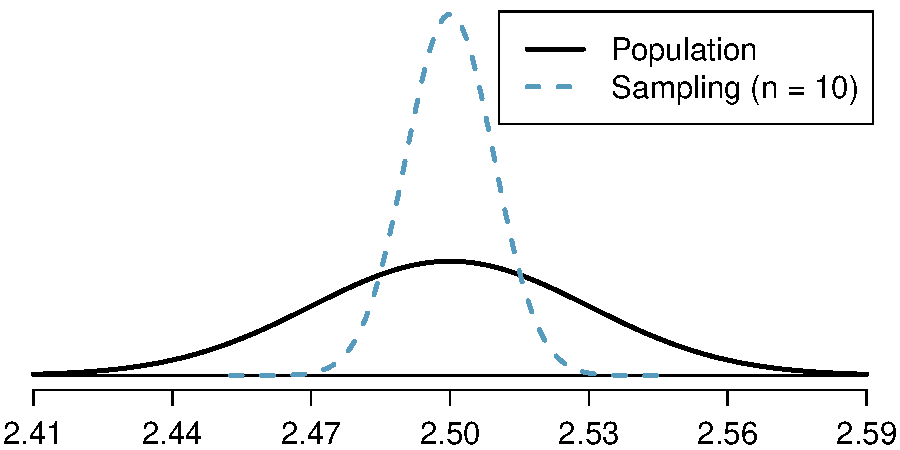
\includegraphics[width=0.48\textwidth]{ch_inference_foundations/figures/eoce/penny_weights/penny_weights_sketch.pdf}
\end{center}
(e)~We could not estimate (a) without a nearly normal population distribution. We also could not estimate (c) since the sample size is not sufficient to yield a nearly normal sampling distribution if the population distribution is not nearly normal.}


\textC{
\end{multicols}
\newpage
\begin{multicols}{2}
}


% 41

\eocesol{(a)~We cannot use the normal model for this calculation, but we can use the
histogram. About 500 songs are shown to be longer than 5 minutes, so the
probability is about $500/3000 = 0.167$.
(b)~Two different answers are reasonable. $^{Option~1}$Since the population
distribution is only slightly skewed to the right, even a small sample size will
yield a nearly normal sampling distribution. We also know that the songs are
sampled randomly and the sample size is less than 10\% of the population, so the
length of one song in the sample is independent of another.  We are looking for
the probability that the total length of 15 songs is more than 60 minutes, which
means that the average song should last at least $60/15 = 4$ minutes. Using
$SD_{\bar{x}}=1.63/\sqrt{15}$, $Z=1.31$ $\to$ 0.0951. $^{Option~2}$Since the
population distribution is not normal, a small sample size may not be sufficient
to yield a nearly normal sampling distribution. Therefore, we cannot estimate
the probability using the tools we have learned so far.
(c)~We can now be confident that the conditions are satisfied.
$Z = 0.92$ $\to$ 0.1788.}

% 43

\eocesol{(a)~$H_0: \mu_{2009} = \mu_{2004}$. $H_A: \mu_{2009} \ne \mu_{2004}$.
(b)~$\bar{x}_{2009} - \bar{x}_{2004} = -3.6$ spam emails per day.
(c)~The null hypothesis was not rejected, and the data do not provide convincing
evidence that the true average number of spam emails per day in years 2004 and
2009 are different. The observed difference is about what we might expect from
sampling variability alone.
(d)~Yes, since the hypothesis of no difference was not rejected in part~(c).}

% 45

\eocesol{(a)~$H_0: p_{2009} = p_{2004}$.  $H_A: p_{2009} \ne p_{2004}$.
(b)~-7\%.
(c)~The null hypothesis was rejected. The data provide strong evidence that the
true proportion of those who once a month or less frequently delete their spam
email was higher in 2004 than in 2009. The difference is so large that it cannot
easily be explained as being due to chance.
(d)~No, since the null difference, 0, was rejected in part (c).}

% 47

\eocesol{True. If the sample size is large, then the standard error will be small,
meaning even relatively small differences between the null value and point
estimate can be statistically significant.}


\end{multicols}
